\documentclass[tikz,border=2pt]{standalone}
\usepackage{amsmath,amssymb}
\usepackage{tikz}
\usetikzlibrary{arrows.meta}

\begin{document}
% Chain rule: the derivative of a composition is the product of the Jacobians, with the sizes
% chaining k x m times m x n = k x n.
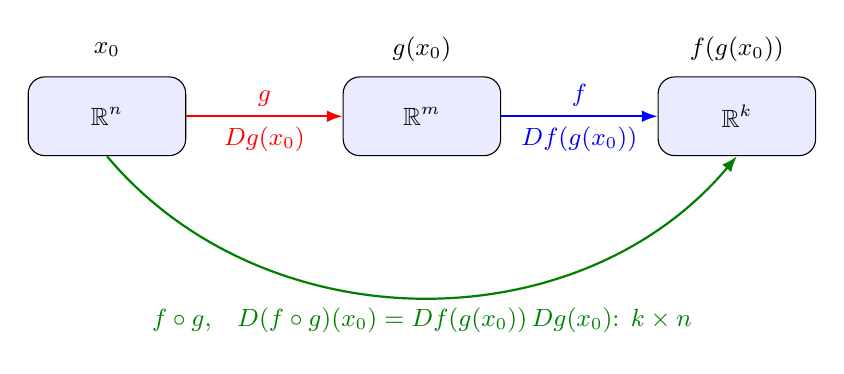
\begin{tikzpicture}[every node/.style={font=\small}, >={Latex[length=2mm]}]
	\node[draw, rounded corners=6pt, fill=blue!8, minimum width=2cm, minimum height=1cm] (A) at (0,0) {$\mathbb{R}^n$};
	\node[draw, rounded corners=6pt, fill=blue!8, minimum width=2cm, minimum height=1cm] (B) at (4,0) {$\mathbb{R}^m$};
	\node[draw, rounded corners=6pt, fill=blue!8, minimum width=2cm, minimum height=1cm] (C) at (8,0) {$\mathbb{R}^k$};
	\draw[->, thick, red] (A) -- (B) node[midway, above] {$g$} node[midway, below, font=\small] {$Dg(x_0)$};
	\draw[->, thick, blue] (B) -- (C) node[midway, above] {$f$} node[midway, below, font=\small] {$Df(g(x_0))$};
	\draw[->, thick, green!50!black] (A.south) to[bend right=50] node[midway, below, font=\small] {$f\circ g$,\quad $D(f\circ g)(x_0)=Df(g(x_0))\,Dg(x_0)$: $k\times n$} (C.south);
	\node[font=\small] at (0,0.85) {$x_0$};
	\node[font=\small] at (4,0.85) {$g(x_0)$};
	\node[font=\small] at (8,0.85) {$f(g(x_0))$};
\end{tikzpicture}
\end{document}
